% Data and method at a glance. Standalone so it can be previewed; the paper includes the compiled PDF.
\documentclass[tikz,border=2pt]{standalone}
\usepackage{times}
\usepackage{amsmath}
\usepackage{booktabs}
\usepackage{array}
\usetikzlibrary{positioning,arrows.meta,calc,backgrounds}
\definecolor{ink}{HTML}{0B0B0B}
\definecolor{ink2}{HTML}{52514E}
\definecolor{rule}{HTML}{C9C8C3}
\definecolor{fillA}{HTML}{EEF4FC}
\definecolor{fillB}{HTML}{FDF0EA}
\definecolor{fillC}{HTML}{EAF7F1}
\definecolor{blue}{HTML}{2A78D6}
\definecolor{orange}{HTML}{EB6834}
\definecolor{aqua}{HTML}{1BAF7A}
\newcommand{\chip}[1]{\tikz[baseline=-0.6ex]\fill[#1] (0,0) rectangle (0.22,0.22);}
\begin{document}
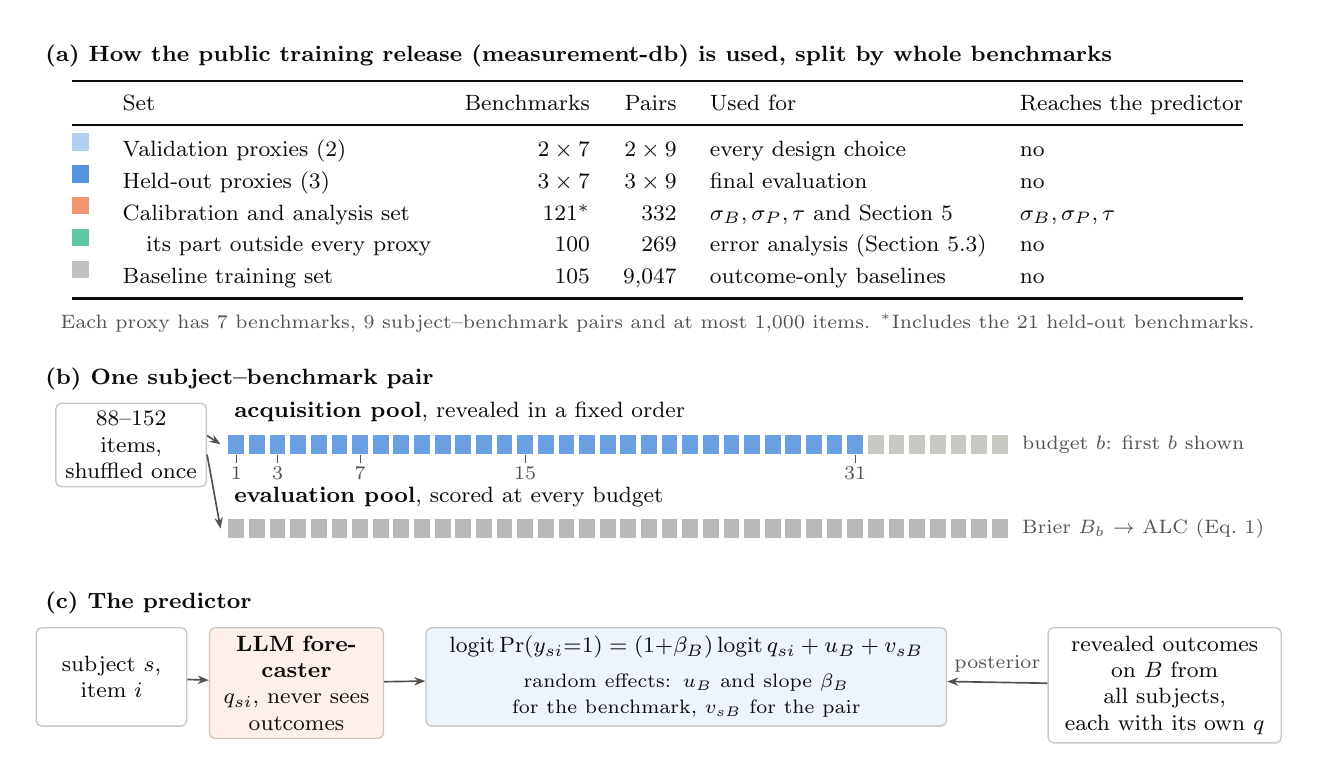
\begin{tikzpicture}[
  font=\footnotesize, text=ink,
  box/.style={draw=rule, rounded corners=2pt, align=center, inner sep=3pt, line width=0.5pt},
  arr/.style={-{Stealth[length=4pt]}, draw=ink2, line width=0.6pt},
  lab/.style={font=\footnotesize\bfseries, anchor=west}
]
% ---------------- (a) uses of measurement-db, as a table ----------------
% The figure spans x = 0 to about 15.8 (the right edge of panel (c)); panel (a) is centred on that width.
\def\CX{7.9}
\coordinate (O) at (0,0);
\node[anchor=north, inner sep=0pt] (tab) at (\CX,0) {%
\renewcommand{\arraystretch}{1.12}%
\begin{tabular}{@{}l l r r l l@{}}
\toprule
 & Set & Benchmarks & Pairs & Used for & Reaches the predictor \\
\midrule
\chip{blue!35} & Validation proxies (2) & $2 \times 7$ & $2 \times 9$ & every design choice & no \\
\chip{blue!80} & Held-out proxies (3) & $3 \times 7$ & $3 \times 9$ & final evaluation & no \\
\chip{orange!70} & Calibration and analysis set & 121$^{\ast}$ & 332 & $\sigma_B, \sigma_P, \tau$ and Section 5 & $\sigma_B, \sigma_P, \tau$ \\
\chip{aqua!70} & \quad its part outside every proxy & 100 & 269 & error analysis (Section 5.3) & no \\
\chip{ink2!35} & Baseline training set & 105 & 9{,}047 & outcome-only baselines & no \\
\bottomrule
\end{tabular}};
\node[lab] at ($(tab.north -| O)+(0,0.3)$) {(a) How the public training release (measurement-db) is used, split by whole benchmarks};
\node[anchor=north, font=\scriptsize, text=ink2] at ($(tab.south)+(0,-0.05)$)
  {Each proxy has 7 benchmarks, 9 subject--benchmark pairs and at most 1{,}000 items. $^{\ast}$Includes the 21 held-out benchmarks.};
% ---------------- (b) one pair ----------------
\coordinate (B) at ($(tab.south -| O)+(0,-1.0)$);
\node[lab] at (B) {(b) One subject--benchmark pair};
% panel (b) content spans about 15.3 of the 15.8 width, so it is shifted right by 0.25 to sit in the centre
\begin{scope}[shift={($(B)+(0.25,0)$)}]
\def\s{0.262}
\def\X{2.2}
\node[box, text width=1.7cm, anchor=north west] (pair) at (0,-0.3) {88--152 items,\\ shuffled once};
\node[anchor=west, font=\footnotesize] at (\X-0.05,-0.42) {\textbf{acquisition pool}, revealed in a fixed order};
\foreach \i in {1,...,31} { \fill[blue!70] ({\X+(\i-1)*\s},-0.95) rectangle ++(0.2,0.24); }
\foreach \i in {32,...,38} { \fill[rule] ({\X+(\i-1)*\s},-0.95) rectangle ++(0.2,0.24); }
\foreach \b in {1,3,7,15,31} {
  \draw[ink2, line width=0.4pt] ({\X+(\b-1)*\s+0.1},-0.97) -- ++(0,-0.1);
  \node[font=\scriptsize, text=ink2] at ({\X+(\b-1)*\s+0.1},-1.2) {\b};
}
\node[font=\scriptsize, text=ink2, anchor=west] at ({\X+38*\s},-0.83) {budget $b$: first $b$ shown};
\node[anchor=west, font=\footnotesize] at (\X-0.05,-1.5) {\textbf{evaluation pool}, scored at every budget};
\foreach \i in {1,...,38} { \fill[ink2!40] ({\X+(\i-1)*\s},-2.02) rectangle ++(0.2,0.24); }
\node[font=\scriptsize, text=ink2, anchor=west] at ({\X+38*\s},-1.9) {Brier $B_b$ $\rightarrow$ ALC (Eq.~1)};
\draw[arr] ($(pair.east)+(0,0.12)$) -- (\X-0.1,-0.83);
\draw[arr] ($(pair.east)+(0,-0.12)$) -- (\X-0.1,-1.9);
\end{scope}
% ---------------- (c) the predictor ----------------
\coordinate (C) at ($(B)+(0,-2.85)$);
\begin{scope}[shift={(C)}]
\node[lab] at (0, 0) {(c) The predictor};
\node[box, text width=1.7cm, anchor=north west, minimum height=1.25cm] (in) at (0,-0.3) {subject $s$,\\ item $i$};
\node[box, fill=fillB, text width=2.0cm, anchor=north west, minimum height=1.25cm] (fc) at (2.2,-0.3) {\textbf{LLM forecaster}\\ $q_{si}$, never sees\\ outcomes};
\node[box, fill=fillA, text width=6.4cm, anchor=north west, minimum height=1.25cm] (model) at (4.95,-0.3)
  {\mbox{$\operatorname{logit}\Pr(y_{si}{=}1) = (1{+}\beta_B)\operatorname{logit} q_{si} + u_B + v_{sB}$}\\[3pt]
   {\scriptsize\hyphenpenalty=10000 random effects: $u_B$ and slope $\beta_B$ for the benchmark, $v_{sB}$ for the pair}};
\node[box, text width=2.75cm, anchor=north west, minimum height=1.25cm] (rev) at (12.85,-0.3)
  {\hyphenpenalty=10000 revealed outcomes\\ on $B$ from all subjects,\\ each with its own $q$};
\draw[arr] (in) -- (fc);
\draw[arr] (fc) -- (model);
\draw[arr] (rev) -- node[above, font=\scriptsize, text=ink2] {posterior} (model);
\end{scope}
\begin{scope}[on background layer]
\fill[white] ($(current bounding box.south west)+(-0.1,-0.1)$) rectangle ($(current bounding box.north east)+(0.1,0.1)$);
\end{scope}
\end{tikzpicture}
\end{document}
